\documentclass[english]{article}
\usepackage[T1]{fontenc}
\usepackage[utf8]{inputenc}
\usepackage{lmodern}
\usepackage[a4paper]{geometry}
\usepackage{babel}
\usepackage{graphicx}
\usepackage{amsmath,amssymb,amsfonts,amsthm,geometry,verbatim,enumerate,float}
\usepackage{tikz}
\usetikzlibrary{shapes.multipart}
\usetikzlibrary{arrows.meta}
\usepackage{caption}
\usepackage{subcaption}
\usepackage{fancyvrb}


\usepackage[%  
	colorlinks=true,
	pdfborder={0 0 0},
	linkcolor=red
]{hyperref}


\begin{document}
	
\title{Shallow description of the Python Virtual Machine \\ \large L3 summer internship}
\author{Mathis Bouverot-Dupuis}
\date{June \& July 2021}

\maketitle 

\begin{figure}[h]
	\centering 
	
\includegraphics[width=.7\linewidth]{img/logoENS.png}	
\end{figure}
\begin{figure}[h]
	\centering 
	
\includegraphics[width=.7\linewidth]{img/logoLORIA.jpg}
\end{figure} 

\newpage 

\tableofcontents
\newpage

\section{Introduction}
This report accounts for the work done under the supervision of Alexandre Talon and Guillaume Bonfante, during June and July of 2021 in the LORIA laboratory (Nancy). Over the course of these two months, I studied the problem of recognizing and describing virtual machines (VMs) from their execution traces.

The context of this study relies on the following issue.
We suppose that we are given an executable for which we must
determine whether it is a malware or not. The problem is that
malware authors try to hide their malware by transforming the code, to make it harder to understand and analyze. Even
if we have the original version of the malware, it is hard (and in general undecidable by Rice's Theorem) to recognize its obfuscated variants.

One of the obfuscation techniques used by malware authors is
to compile their binary code with a virtual machine,
see \cite{surreptsoft}.

A virtual machine is given by a (usually low level) language (next named bytecode) together with its semantics,
usually described by an interpreter for the language. The basis of the
obfuscation is then to compile the malware's source code to the bytecode language and
to embark both the interpreter and the obfuscated code within the malware executable.

Some packers such as VMProtect (see \cite{vmprotect}) will perform such an operation.

A VM is an abstract version of a computer system: it is a program that reads a list of instructions (in a format called bytecode) and executes them. Its design is based on that of physical machines. The execution of an instruction consists of the following steps:
\begin{enumerate}
	\item Fetch: reads the instruction from memory.
	\item Decode: parses the instruction. If the instruction is formatted in a typical way, it is divided into an opcode followed by zero or more arguments (similar to machine code).
	\item Dispatch: based on the opcode, decides which code (or function) to run.
	\item Execute: carries through the semantics of the instruction. This is where the VM's internal state is updated and input/output operations are performed.
\end{enumerate}
The serial execution of several instructions forms the VM loop (see Figure \ref{fig:abstractVM:Centralized}).

% Context + other papers
During this internship my goal was, broadly speaking, to reverse engineer a VM: I would observe the execution of a VM and first try to detect that it is a VM, then try to find out what it is doing. Similar work has been done in the context of binary deobfuscation: a popular technique to hide the original source code of a program (\textit{i.e.} obfuscate it) is to translate parts of it into some proprietary bytecode to be interpreted at run-time by a virtual machine. This protection can however be bypassed, as shown by Salwan, Bardin and Potet in \cite{tritondeobfs}. They used the Triton dynamic binary instrumentation framework along with the powerful techniques it enables such as taint analysis and symbolic execution to find the original source code (or an equivalent code) of obfuscated programs. Unlike traditional `by hand' reverse-engineering techniques, which first try to understand the proprietary bytecode before finding the source code, they leveraged Triton to find the source code without having to find much about the VM. 

I studied a specific class of VMs: programming language interpreters. Typical examples include the Python interpreter and the Java Virtual Machine. I focused on two Python interpreters: CPython \cite{cpython} and PyPy \cite{pypy}. My approach was more lightweight than the one of Salwan et al. Without using heavy techniques and only using the fact that the Python interpreter is a VM, my goal was to:
\begin{enumerate}
	\item Find the bytecode of the program being run.
	\item Find some level of semantics about the bytecode.
\end{enumerate}

The first step was to analyze the trace of an execution of a Python interpreter to find the VM loop. Then I had to find the main parts of the VM state such as the program bytecode, the instruction pointer ($ip$), the stack pointer ($sp$), and so on. Finally I observed how each Python instruction changes the state of the VM to reconstruct some basic level of semantics about the Python opcodes.

\section{Recognizing the VM execution}

We will now describe in more details our starting point. We give ourselves a VM to analyze (for instance the CPython interpreter). We assume that we do not have access to the source code or to the machine code of the VM executable. What we do allow ourselves to use is the execution trace of single runs of the VM: the ordered list of machine instructions the VM executable uses to run a given program. Note that this does not give us access to the complete machine code of the VM executable, nor to the bytecode instructions of the program the VM runs. 

I obtained this execution trace using a custom Intel Pin tracer \cite{intelpin}. Writing the Pintool was a non-trivial task: I had to balance several challenges such as memory consumption (we have to store information about every noteworthy machine instruction that is executed, which can quickly add up to gigabytes of data), execution time (running a program instrumented with Pin is several orders of magnitudes slower than normal) and unclear parts of the Pin user guide.

The first step to analyze the VM is thus to recognize it in the execution trace: can we recognize the fetch-decode-dispatch-execute pattern? In what follows we will often write `finding the fetch' to avoid repeating `fetch-decode-dispatch'.

\subsection{Building the CFG}

We start by building the control flow graph (CFG) from the VM trace. We group instructions by basic blocks: a sequence of instructions that has only one entry point and one exit point, and build a graph whose vertices are basic blocks and whose edges indicate branches taken during the execution.

More precisely: for a machine instruction $I$, we call $next(I)$ (resp. $prev(I)$) the set of instructions that, at some point of the execution, immediately follow (resp. precede) $I$ in the execution trace. A basic block is then an ordered list of instructions $I_1 \dots I_n$ such that $\forall k, next(I_k) = \{I_{k+1}\} \textrm{ and } prev(I_{k+1}) = \{I_k\}$. Note that two consecutive instructions in a basic block do not have to be consecutive in memory (example: an unconditional branch). 

We then build a graph on the basic blocks. We add an edge from a block $I_1 \dots I_n$ to a block $J_1 \dots J_p$ if and only if $J_1 \in next(I_n)$, which is equivalent to $I_n \in prev(J_1)$.

As the size and complexity of CFGs built this way grow very fast, we apply some additional transformations to simplify the graph. Each time we see a \texttt{call} instruction, we find the corresponding \texttt{ret} instruction, and delete and add edges as shown in Figure \ref{fig:callRet}. This transformation requires that all \texttt{call} instructions have a matching \texttt{ret} instruction. This is not always the case with malware: programs can use call stack tampering and (ab)use \texttt{call} instructions for other purposes. However I believe this is not a fundamental limitation of this approach : with more effort and time this method could probably be adapted to work even with call stack tampering.

As a consequence of this transformation, the CFG is split into several connected components, each corresponding to a single function (this is the convention adopted by the binary analysis framework IDA).

\begin{figure}[htp]
	\centering
	\begin{subfigure}{.5\textwidth}
		\centering 	
		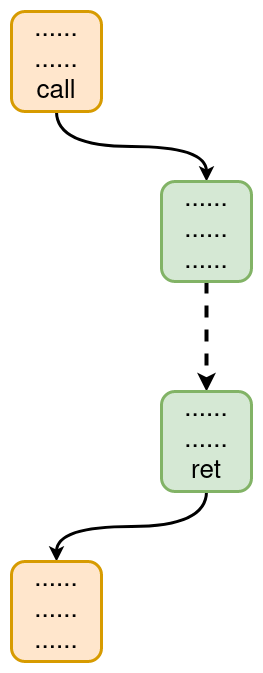
\includegraphics[width=.4\linewidth]{img/CallRetBefore.png}
		\caption{Original CFG}
	\end{subfigure}%
	\begin{subfigure}{.5\textwidth}
		\centering 	
		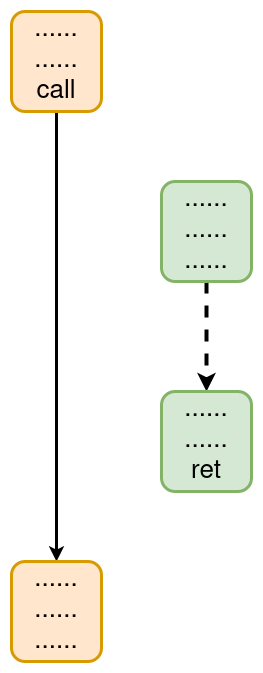
\includegraphics[width=.4\linewidth]{img/CallRetAfter.png}
		\caption{Transformed CFG}
	\end{subfigure}
	
	\caption{Transformation of the CFG around call/ret. The full arrows represent edges in the CFG. The dashed arrow indicates that there may be other blocks between the two green blocks. These other blocks are not modified.}
	\label{fig:callRet}
\end{figure}
 
\subsection{Finding the fetch}

\subsubsection{Basic Method}

The basic idea to find the fetch is to assume that all opcodes share the same basic block for the fetch, as in Figure \ref{fig:abstractVM:Centralized}.
Note that this is a somewhat restrictive assumption, albeit necessary for this method to work. Some VM implementations use a fetch block for each different opcode (see Figure \ref{fig:abstractVM:Decentralized}): most notably CPython does so. This optimization (`computed-gotos') can thankfully be disabled when compiling CPython. In all my experiments I used this modified CPython version.

\begin{figure}[htp]
	\centering
	\begin{subfigure}{.5\textwidth}
		\centering 	
		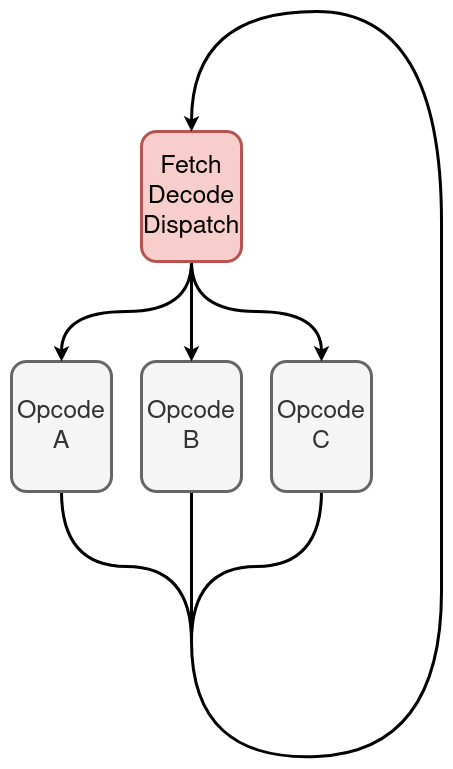
\includegraphics[width=.7\linewidth]{img/FetchCentralized.png}
		\caption{Centralized fetch}
		\label{fig:abstractVM:Centralized}
	\end{subfigure}%
	\begin{subfigure}{.5\textwidth}
		\centering 	
		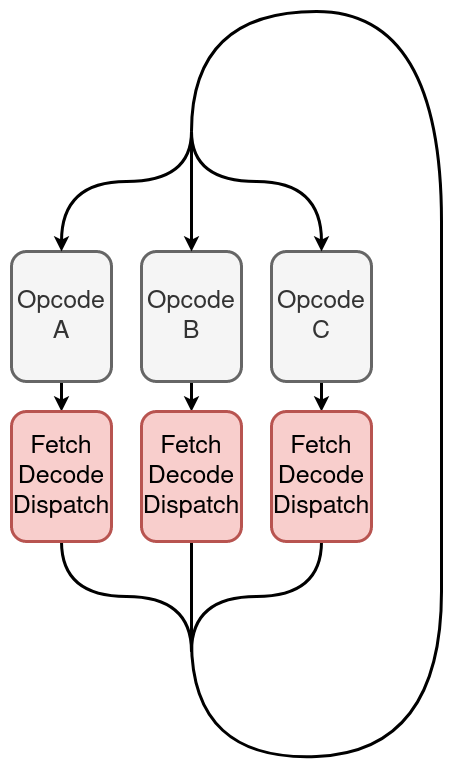
\includegraphics[width=.7\linewidth]{img/FetchDecentralized.png}
		\caption{Decentralized fetch (`computed-gotos')}
		\label{fig:abstractVM:Decentralized}
	\end{subfigure}
	\caption{Examples of VM control flow graphs}
	\label{fig:abstractVM}
\end{figure}

We thus build the CFG $\mathcal{C}$ and look for a basic block that:
\begin{itemize}
	\item is executed a large number of times (because it is shared between all opcodes).
	\item contains at least one instruction that reads a few bytes from memory (the fetch).
	\item has a large number of outgoing edges (the dispatch).
\end{itemize} 

Unfortunately, this method is too restrictive: the fetch, decode and dispatch are not always in the same basic block in $\mathcal{C}$ (see Figure \ref{fig:concreteVMOriginal}). There can be branches (e.g. to check for a termination condition, and so on) between the fetch and the dispatch. 

\subsubsection{Using the filtered CFG}

To handle this issue, we first filter out details from $\mathcal{C}$, and then hope that the fetch-decode-dispatch are in the same basic block in the new CFG $\mathcal{C}_{filtered}$. 

When building $\mathcal{C}_{filtered}$, we want to remove blocks that are executed very rarely. Even between blocks that are executed a lot, we also want to remove edges that are executed very rarely. More formally, given two parameters $exec\_blocks$ and $exec\_edges$, we build $\mathcal{C}_{filtered}$ as follows: 
\begin{itemize}
	\item For each block $B \in \mathcal{C}$, if $B$ is executed at least $exec\_blocks$ times, add $B$ to $\mathcal{C}_{filtered}$.
	\item For each edge $(E: B \rightarrow B') \in \mathcal{C}$, if $E$ is executed at least $exec\_edges$ times and both $B$ and $B'$ are executed at least $exec\_blocks$ times, add $E$ to $\mathcal{C}_{filtered}$.
\end{itemize}
We then apply a simple transformation on $\mathcal{C}_{filtered}$ to merge all blocks $B$ and $B'$ such that $next(B) = \{B'\}$ and $prev(B') = \{B\}$. In the experiments I had to tune the values of $exec\_blocks$ and $exec\_edges$, and found values around $1000$ to give satisfactory results. This method thus only works on Python programs that contain at least a few thousand bytecode instructions. The number of bytecode instructions for a given program can sometimes be larger than expected: interpreters execute some initialization and finalization bytecode in addition to the main program. In the case of PyPy the number of additional bytecode instructions is large enough that even trivial Python programs can be successfully analyzed, however in the case of CPython we will not be able to detect the VM loop in very small Python programs.

The CFG $\mathcal{C}_{filtered}$ only retains the main structure of the graph, abstracting away the code paths rarely taken: see Figures \ref{fig:concreteVMFiltered} and \ref{fig:concreteVMOriginal} for a comparison between $\mathcal{C}$ and $\mathcal{C}_{filtered}$. Since $\mathcal{C}_{filtered}$ can miss parts of or most of the opcode execution code, the original CFG $\mathcal{C}$ is a good place to look for the dispatch. However in $\mathcal{C}$, the fetch, decode and dispatch may not be in the same basic block : we look in $\mathcal{C}_{filtered}$ for a block containing all three.

We thus look for a basic block in $\mathcal{C}_{filtered}$ that:
\begin{itemize}
	\item is executed a large number of times.
	\item contains at least one instruction that reads a few bytes from memory (the fetch).
	\item contains at least one instruction that has a large number of outgoing edges in $\mathcal{C}$.
\end{itemize}

Once we have found the fetch, it is easy to find the bytecode: we simply get the value read by the fetch. We can also divide the trace into chunks corresponding to each bytecode, and remove the irrelevant parts of the VM trace (initialization and finalization code): we then obtain a list of small traces for each opcode.

\begin{figure}[htp]
	\centering 
	\begin{subfigure}{.5\textwidth}
		\centering 	
		\begin{BVerbatim}
f = open("file", "w")
for i in range(1000):
	f.write(str(i))
		\end{BVerbatim}
		\caption{Python source code.}
		\label{fig:examplePythonProg:source}
	\end{subfigure}%
	\begin{subfigure}{.5\textwidth}
		\centering 	
		\begin{BVerbatim}
LOAD_NAME                0 (open)
LOAD_CONST               0 ('file')
LOAD_CONST               1 ('w')
CALL_FUNCTION            2
STORE_NAME               1 (f)
LOAD_NAME                2 (range)
LOAD_CONST               2 (1000)
CALL_FUNCTION            1
GET_ITER
FOR_ITER                18 (to 38)
STORE_NAME               3 (i)
LOAD_NAME                1 (f)
LOAD_METHOD              4 (write)
LOAD_NAME                5 (str)
LOAD_NAME                3 (i)
CALL_FUNCTION            1
CALL_METHOD              1
POP_TOP
JUMP_ABSOLUTE           18
LOAD_CONST               3 (None)
RETURN_VALUE
		\end{BVerbatim}
		\caption{Disassembled bytecode.}
		\label{fig:examplePythonProg:bytecode}
	\end{subfigure}
	\caption{An toy python program, used to generate the graphs in Figures 	\ref{fig:concreteVMFiltered} and \ref{fig:concreteVMOriginal}, along with its disassembly as given by Python's `dis' module.}
	\label{fig:examplePythonProg}
\end{figure}

\begin{figure}[htp]
	\centering 	
	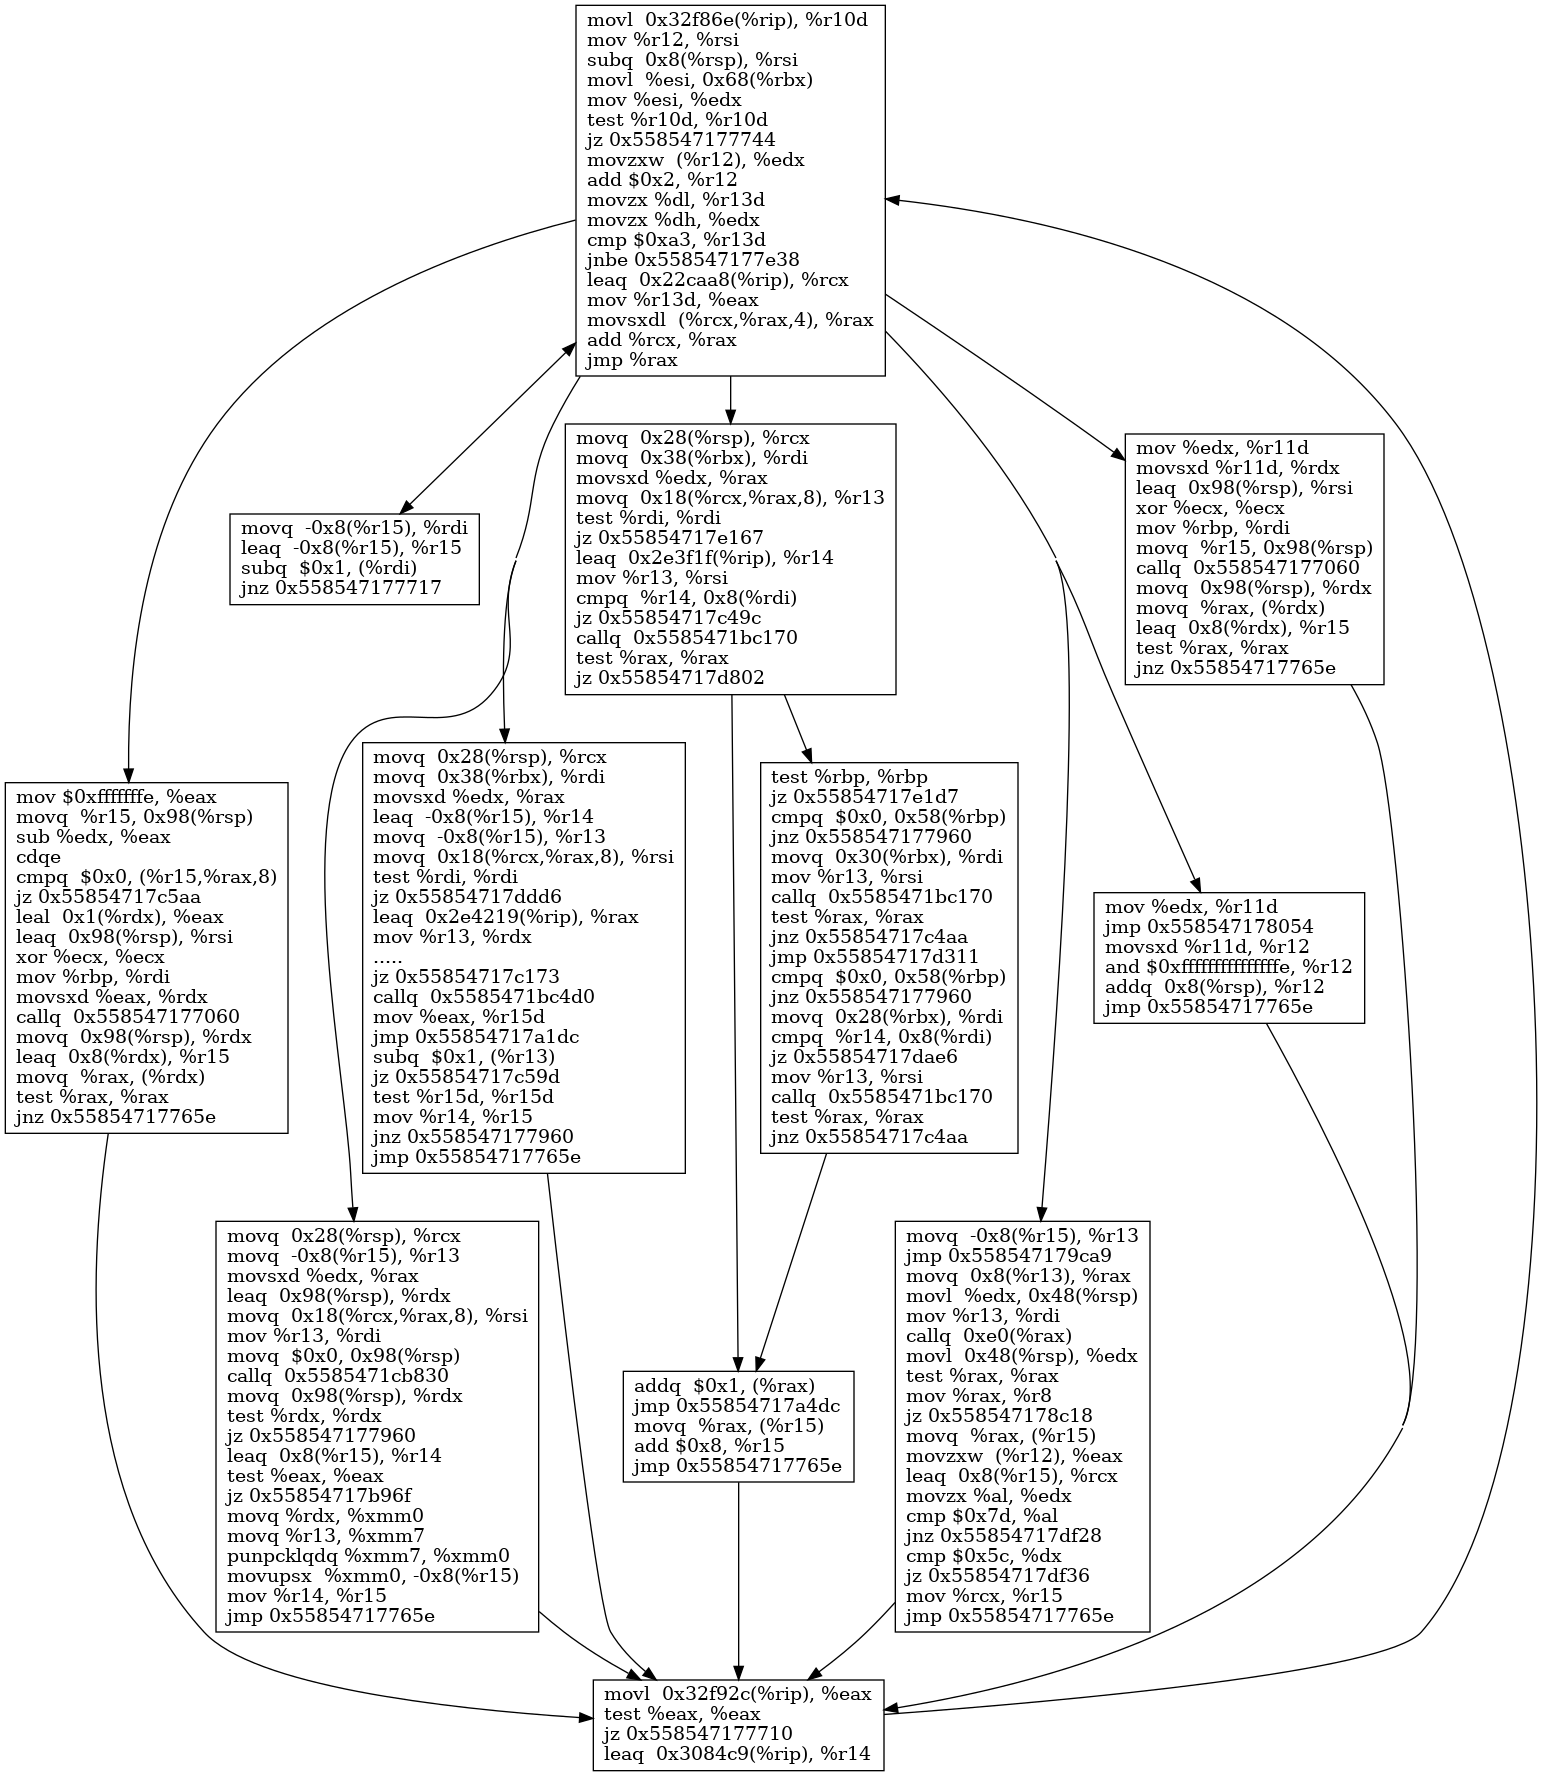
\includegraphics[width=\linewidth]{img/ConcreteVMFiltered.png}
	\caption{The function implementing the VM loop in $\mathcal{C}_{filtered}$, constructed from a trace of CPython running the program in Figure \ref{fig:examplePythonProg}. Notice how the fetch `\texttt{movzxw (\%r12), \%edx}' and the dispatch `\texttt{jmp \%rax}' are in the same block (the topmost block), and that this block has relatively few outgoing edges.}
	\label{fig:concreteVMFiltered}
\end{figure}

\begin{figure}[htp]
	\centering 	
	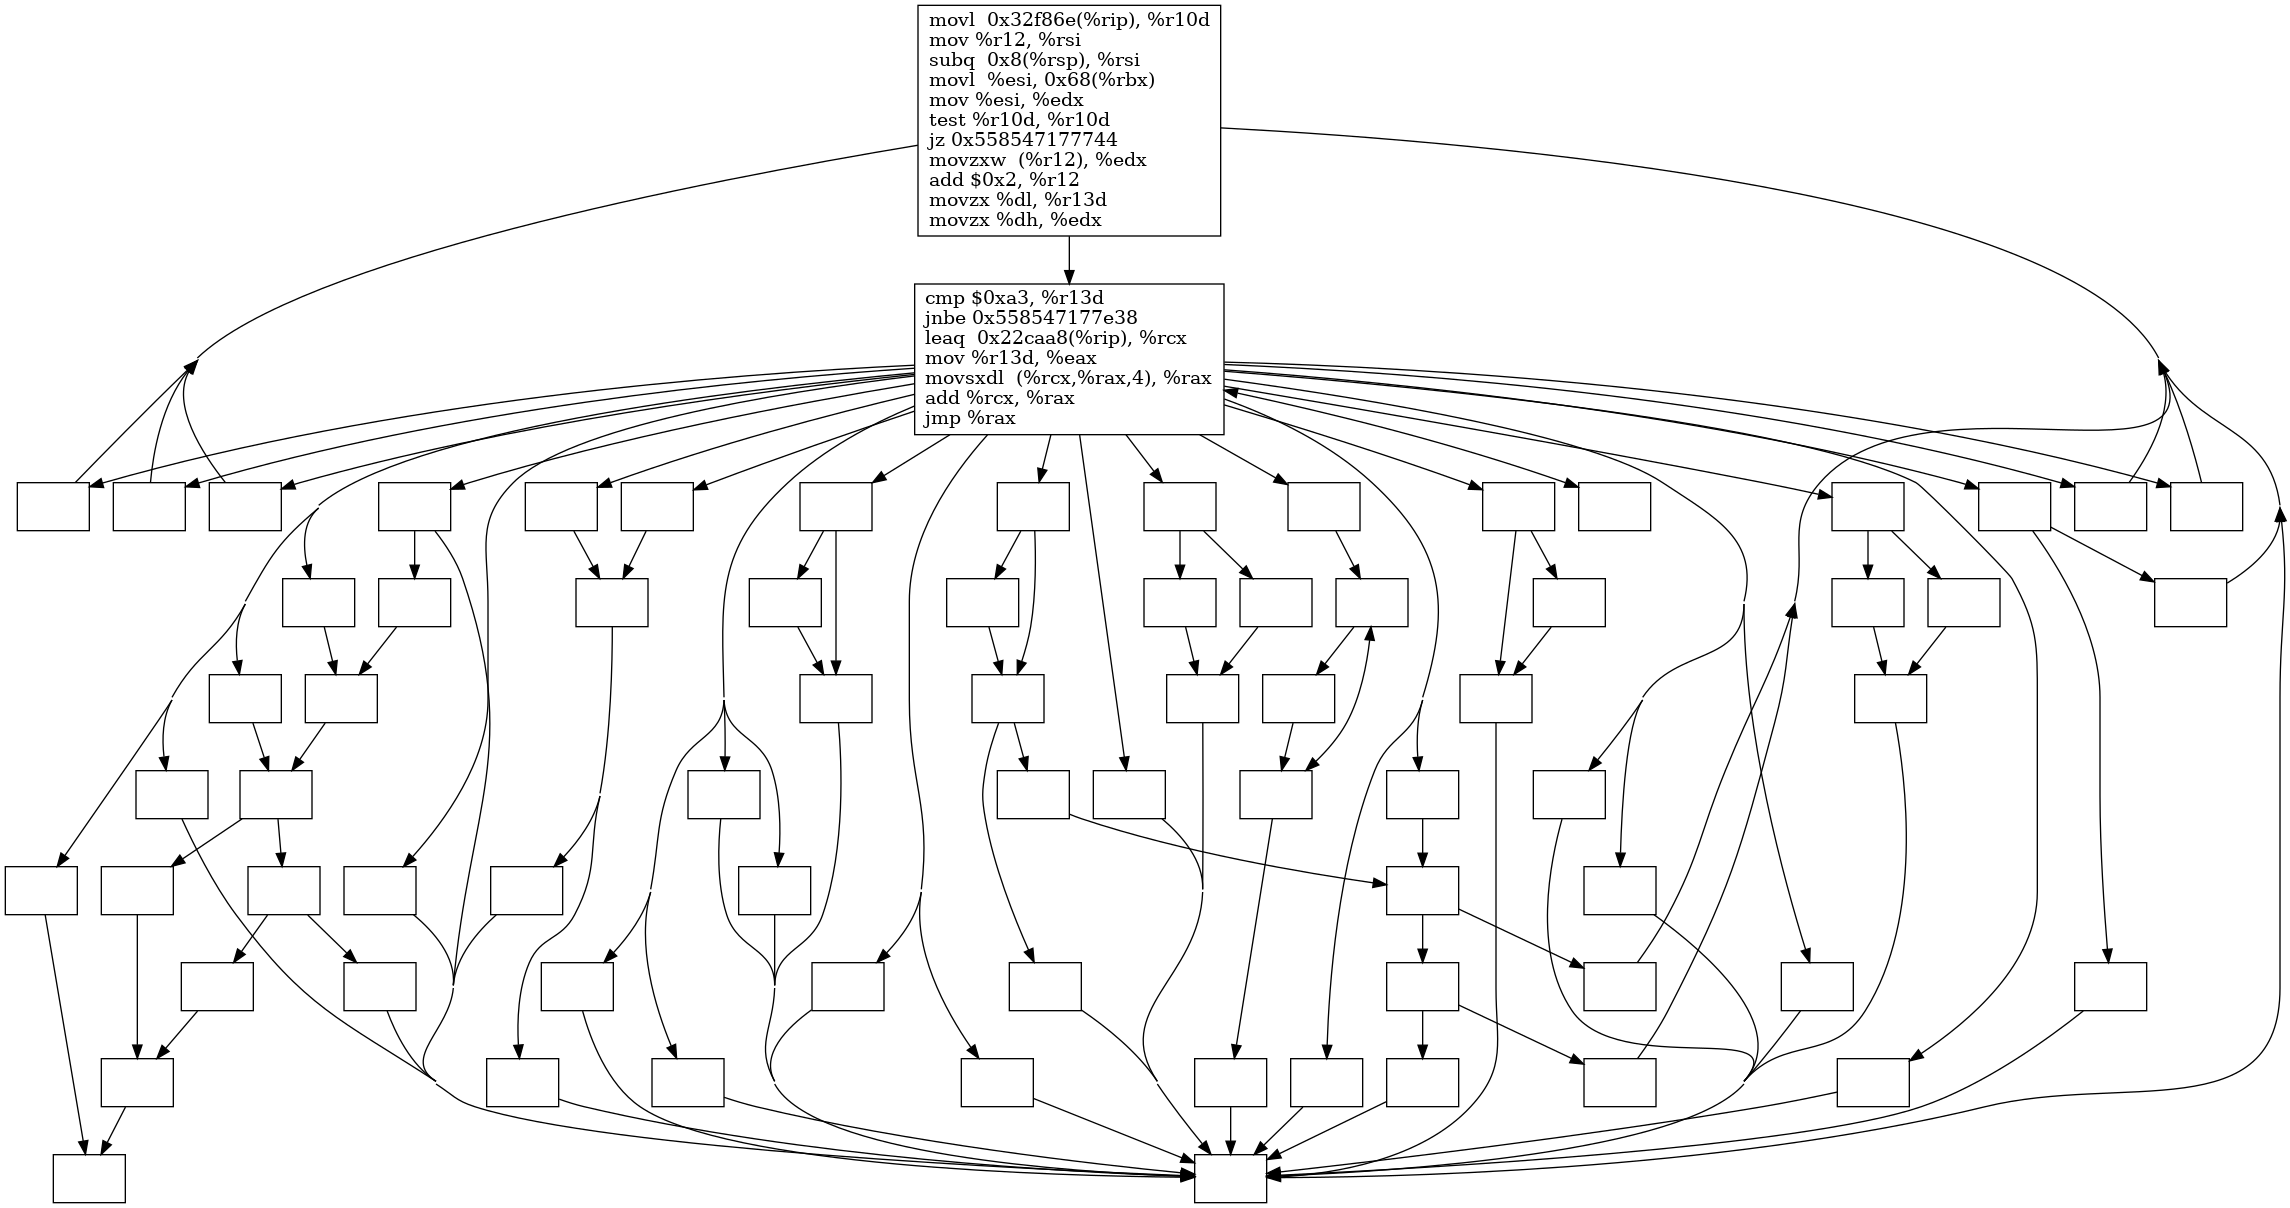
\includegraphics[width=\linewidth]{img/ConcreteVMOriginal.png}
	\caption{The function implementing the VM loop in $\mathcal{C}$, constructed from the same trace as in Figure \ref{fig:concreteVMFiltered}. Only the blocks implementing the fetch and the dispatch have their code shown. Notice how the fetch and the dispatch are in different blocks, and that the dispatch has many outgoing edges.}
	\label{fig:concreteVMOriginal}
\end{figure}

\section{Abstract VM model}

Before we can continue the analysis any further, we give ourselves an abstract VM model. While the previous section does not assume much about the VM, this model follows more closely the Python VM.
\subsection{Definition}

We assume we are working with a stack-based VM, with no general-purpose registers (it does however have `registers' such as $ip$, the instruction pointer). Its internal state consists of:
\begin{itemize}
	\item a set of code blocks 
	\item a set of value stacks 
	\item a stack of frames.  
	\item pointers to the current frame ($fp$: frame pointer), the current bytecode instruction ($ip$: instruction pointer) and the top of the current value stack ($sp$: stack pointer)
\end{itemize}

A code block is a list of bytecode instructions. Each instruction is 2 bytes wide, the first byte being the opcode (as an example, CPython uses $23$ for BINARY\_ADD, $1$ for POP\_TOP, $113$ for JUMP\_ABSOLUTE, and so on) and the second byte being an argument. All instructions have an argument byte, even those that don't use it. A code block contains all the code a given Python function can execute.

A value stack is a stack of Python values (objects). The contents of the stack are opaque to us. However all the values in the stack are contiguous in memory and of the same size.

Each frame corresponds to the execution of some Python function. A frame has its own code block and value stack.

The term `pointer' is intentionally vague: a pointer could be stored in a physical register (\texttt{\%rax}, \texttt{\%rbx}, and so on) or in a memory cell, it may contain the address of the object it points to or be an index into a list. In the experiments I ran, I had to make additional assumptions about pointers, as will be explained in the following section.

We will write $ptr \leftarrow f(ptr)$ where $f$ is any function and $ptr$ is $ip$, $sp$ or $fp$ to indicate that a given opcode changes the value of $ptr$ to $f(ptr)$.

\subsection{Finding the VM state}

We assume that the state of the VM is valid at the fetch/dispatch block. At other points in the execution trace, the registers and memory cells used to store the VM state may be used for different purposes. Our goal is then to find as much information as we can about the VM state before each bytecode instruction is fetched.

\subsubsection{Finding $ip$}

Our method to find the fetch (using the CFG) gives us the machine instruction(s) that read the Python bytecode instruction (in Figure \ref{fig:concreteVMFiltered}, there is one instruction that reads the Python instruction : it is `\texttt{movzxw (\%r12), \%edx}'). Using the Pin tracer, we can find the memory address that is read from: this is the value held by $ip$ at this point. If we then use the Pin tracer to get the two bytes at this address, we also have the Python instruction that is being executed.

\subsubsection{Finding $fp$}

% todo : explain more about the C stack
To find the frame pointers, we must make another assumption: that the C stack of the interpreter corresponds to the stack of the Python program it is running (remember we only look at the program state between bytecodes). Changes in \texttt{\%rsp} should then give us the points at which the frame changes. Looking at registers that also change exactly at the same time as \texttt{\%rsp} (and are also aligned on 8 bits) gives us additional frame pointers: pointers to some frame data (for instance, a C struct on the heap).

Knowing the values of the frame pointers, we then tried to recognize the stack structure of frames, but some opcodes seem to operate on the frame stack in non-standard ways, \textit{i.e.} other than pushing or poping one or several frames. This was a limitation that prevented us from working much with opcodes that deal with frames, such as CALLs and RETs, as will be explained later on.

\subsubsection{Finding $sp$}

A first challenge is where to look for $sp$: registers or memory? It turns out it can be in both, depending on the interpreter: in a register for CPython, in memory for PyPy. Looking for $sp$ in registers is straightforward, as there are a very limited number of them. However memory is more complex: we can not scan through each memory cell. What we can hope for is that $sp$ is stored in a C struct pointed to by a frame pointer: $sp$ must be used very often, so requiring more than one pointer indirection to access it seems very inefficient. We thus look for $sp$ near addresses pointed to by frame pointers.  More precisely, we assume $sp$ will always be stored at $[fp + cte]$ where $fp$ is a frame pointer (whose value can change during the program execution) and $cte$ is a small constant offset (a multiple of 8 bits).

To detect whether a location (register or memory cell) stores the value of $sp$, we take the list of values this location holds for each opcode. The basic idea is that many opcodes modify $sp$ in the same way: pop or push a few values. But we must be careful: we do not know whether $sp$ is stored as the address of the top stack cell, or as the index of the top stack cell, or something else. Depending on the case, a PUSH might increment $sp$ by $8$, $1$ or something else. The solution is to compute the alignment of $sp$, \textit{i.e.} the largest power of $2$ that divides all the values in the list. We implement this idea as:
\begin{itemize}
	\item Compute the maximum consecutive number of times that $sp \leftarrow sp + k*align$ where $k$ is a small constant (e.g. $-2 \leq k \leq 2$). This number should not change much with the size of the program (we check consecutive occurences): we require it to be larger than a constant (e.g. $10$).
	\item Compute the maximum (not necessarily consecutive) number of times that $sp \leftarrow sp - align$, \textit{i.e.} the number of POPs. This number should be proportional to the size of the program: we check it is larger than a percentage of the total opcode count (e.g. $10\%$).
\end{itemize}
The second test used is to distinguish between $sp$ and $ip$/$fp$: $ip$ and $fp$ might be stored in a similar way as $sp$, and pass the first test. 

\subsubsection{Code blocks}

We compute the code blocks by partitioning the bytecode instructions according to (the transitive closure of) the following relation. Two bytecode instructions are in the same code block if:
\begin{itemize}
	\item They are executed in the same frame (\textit{i.e.} there is no frame change between two of their executions). This is because all instructions executed inside a frame are in the same Python function.
	\item They are close in memory. This is because different code blocks are likely to be far apart in memory. % todo: why?
\end{itemize}


\section{Opcode semantics}

\subsection{Examples}

% todo : blabla d'intro (cf. notes d'Alexandre)
Once we have the values of $ip$ and $sp$ for each opcode, we try to attribute semantics to each opcode, \textit{i.e.} characterize how they change the values of $ip$ and $sp$. One limitation of our `shallow' description is that we do not know what values are stored on the stack: typical Python interpreters use the stack to store pointers to objects whose memory layout we do not know. We thus can not differentiate between an BINARY\_ADD and a BINARY\_MUL operation for instance. All we can detect is the number of push/pop each opcode performs and how it changes the value of $ip$.

We would like to build semantics of the following form, e.g. for the simple case of a BINARY\_ADD opcode:
\begin{itemize}
	\item $ip \leftarrow ip + 2$
	\item $sp \leftarrow sp - 8$
\end{itemize}
This means that when we execute this opcode, $ip$ always increases by $2$ and $sp$ always decreases by $8$ (BINARY\_ADD pops its two arguments, pushes the result and advances to the next instruction). Recall that Python instructions are $2$ bytes long, so $ip + 2$ is the instruction directly following $ip$. However $sp$ can be the address of the top of the stack, in which case $sp - 8$ is the value directly under $sp$, since stack values are $8$ byte pointers, or can be something else. If it is for example an index in a list, $sp$ will be aligned on $1$ rather than on $8$, and BINARY\_ADD would have the following semantics:
\begin{itemize}
	\item $ip \leftarrow ip + 2$
	\item $sp \leftarrow sp - 1$
\end{itemize}
Likewise, one could imagine a Python interpreter that grows the stack towards the bottom (CPython and PyPy both grow the stack towards the top), in which case it could become $sp \leftarrow sp + 1$. The precise semantics of an opcode can thus depend on the particular interpreter we choose, and indeed CPython and PyPy have such differences.

Another characteristic of our approach is that a single execution trace often does not give us enough information to find the most general semantics for opcodes that have non-trivial effects on $ip$ and $sp$. Take for example a conditional jump instruction such as POP\_JUMP\_IF\_TRUE, which performs a jump if the top of the stack is \texttt{true} and otherwise advances to the next instruction. In a trace where both cases (\texttt{true} and \texttt{false}) are encountered, we are able to correctly classify it as a conditional jump. However if each time we see this opcode the top of the stack is \texttt{false}, we are not able to detect that this is a conditional jump (or even a jump) and must give it the semantic $ip \leftarrow ip + 2$. The precision of our semantics is thus limited by the given execution trace we use.

Note that for a given opcode, several semantics may be acceptable. For instance the BINARY\_ADD opcode does not need an argument, and CPython has the convention to always set the argument byte to $0$ in this case: we could characterize this opcode by $ip \leftarrow ip + 2$ as well as by $ip \leftarrow ip + arg + 2$. In the second case we would interpret it as a relative jump, which it obviously is not. I thus had to choose which characterization to give for each opcode when several are acceptable.

\subsection{Definition}

Building the $ip$-related semantics of an opcode is relatively straightforward. Most opcodes never change the current frame. For these, we give one of the following characterizations:
\begin{enumerate}
	\item Fall-through: $ip \leftarrow ip + k$. This corresponds to opcodes that do not alter the control-flow of the program.
	\item Relative jump: $ip \leftarrow ip + arg + k$.
	\item Absolute jump: $ip \leftarrow \textrm{block-start} + arg + k$.
	\item Conditional jump: $\textrm{either } ip \leftarrow ip + k_1 \textrm{ or } ip \leftarrow \textrm{block-start} + arg + k_2$. Note that we cannot find what the condition is, since this would require us to inspect the values in the stack, which as we mentioned earlier are opaque.
\end{enumerate}
Here $k$, $k_1$ and $k_2$ are small constants (typically $-2 \leq k, k_1, k2 \leq 2$), $arg$ is the value of the argument byte of the opcode, and `\texttt{block-start}' is the address of the first instruction in the current code block. 	
In the list just above, the characterizations are listed (top to bottom) from the most `general' to the most precise: for each opcode, we give it the most `general' characterization that is acceptable.

We did not manage to find much about instructions that jump between frames, for lack of proper frame identification (we only know when frames change, not what frame we are in). We thus did not characterize CALL or RET instructions. One additional difficulty is that CALL-like Python instructions do not always correspond to a change of frame. They are sometimes (but not always) handled internally by the interpreter (e.g. calls to internal libraries such as I/O functions): the next opcode in the trace is thus the fall-through instruction, and no frame change has been made.

Building the $sp$-related semantics is similar. Again, dealing with opcodes that change the current frame is too difficult, but for those that never change it, we give one of the following characterizations (from the most general to the least):
\begin{enumerate}
	\item $sp \leftarrow sp + k$. This corresponds to most simple pop/push opcodes, as well as most binary operations (ADD, SUB, MUL, \dots).
	\item $sp \leftarrow sp \pm A*arg + k$. This corresponds to opcodes that either consume a number of values given by $arg$ (e.g. BUILD\_TUPLE) or produce a number of values given by $arg$ (e.g. UNPACK\_SEQUENCE).
\end{enumerate}
Here $k$ is a small constant (typically $-2 \leq k \leq 2$), $arg$ is the value of the argument of the opcode, and $A$ is the alignment of $sp$ (typically $1$ or $8$).

An exemple of the semantics we are able to compute is given in Figure \ref{fig:semanticsTable}. Notice that this table contains more distinct opcodes than the Python program it was built from (Figure \ref{fig:examplePythonProg}): this is because interpreters execute some initialization and finalization bytecode before and after the program's bytecode. Conversely, some opcodes in the python program do not appear in the table or have an incomplete characterization (e.g. EXTENDED\_ARGS): our simple model does not allow us to give a characterization for all opcodes, and most notably for opcodes that change the frame (e.g. CALL\_FUNCTION and RET). Another interesting opcode is POP\_JUMP\_IF\_FALSE: we would expect it to be classified as a conditional jump. However every time this opcode was executed, the same branch was taken, and our model thus classifies it as an absolute jump.

\begin{figure}[htp]
	\centering
	\begin{tabular}{|c|c|c|}
		\hline
		POP\_TOP & $ip \leftarrow ip + 2$ & $sp \leftarrow sp - 8$\\
		\hline
		BUILD\_SLICE & $ip \leftarrow ip + 2$ & $sp \leftarrow sp - 8$\\
		\hline
		UNARY\_NEGATIVE & $ip \leftarrow ip + 2$ & $sp \leftarrow sp + 0$\\
		\hline
		CALL\_FUNCTION\_KW & $ip \leftarrow ip + 2$ & $sp \leftarrow sp - 8*arg - 8$\\
		\hline
		EXTENDED\_ARG & $ip \leftarrow ip + 4$ & \\
		\hline
		BINARY\_SUBTRACT & $ip \leftarrow ip + 2$ & $sp \leftarrow sp - 8$\\
		\hline
		BINARY\_SUBSCR & $ip \leftarrow ip + 2$ & $sp \leftarrow sp - 8$\\
		\hline
		FORMAT\_VALUE & $ip \leftarrow ip + 2$ & $sp \leftarrow sp + 0$\\
		\hline
		BUILD\_STRING & $ip \leftarrow ip + 2$ & $sp \leftarrow sp - 8$\\
		\hline
		LOAD\_METHOD & $ip \leftarrow ip + 2$ & $sp \leftarrow sp + 8$\\
		\hline
		CALL\_METHOD & $ip \leftarrow ip + 2$ & $sp \leftarrow sp - 8*arg - 8$\\
		\hline
		BINARY\_AND & $ip \leftarrow ip + 2$ & $sp \leftarrow sp - 8$\\
		\hline
		GET\_ITER & $ip \leftarrow ip + 4$ & $sp \leftarrow sp + 8$\\
		\hline
		POP\_BLOCK & $ip \leftarrow ip + 2$ & $sp \leftarrow sp + 0$\\
		\hline
		STORE\_NAME & $ip \leftarrow ip + 2$ & $sp \leftarrow sp - 8$\\
		\hline
		STORE\_ATTR & $ip \leftarrow ip + 2$ & $sp \leftarrow sp - 16$\\
		\hline
		LOAD\_CONST & $ip \leftarrow ip + 2$ & $sp \leftarrow sp + 8$\\
		\hline
		LOAD\_NAME & $ip \leftarrow ip + 2$ & $sp \leftarrow sp + 8$\\
		\hline
		LOAD\_ATTR & $ip \leftarrow ip + 2$ & $sp \leftarrow sp + 0$\\
		\hline
		JUMP\_FORWARD & $ip \leftarrow ip + arg + 2$ & $sp \leftarrow sp + 0$\\
		\hline
		JUMP\_ABSOLUTE & $ip \leftarrow \textrm{ block-start } + arg + 0$ & $sp \leftarrow sp + 0$\\
		\hline
		POP\_JUMP\_IF\_FALSE & $ip \leftarrow \textrm{ block-start } + arg + 0$ & $sp \leftarrow sp - 8$\\
		\hline
		POP\_JUMP\_IF\_TRUE & 
		$ip \leftarrow 
		\left\{ 
		\begin{array}{ll}
		ip + 2 \\ 
		\textrm{block-start } + arg + 0
		\end{array}
		\right.$ & $sp \leftarrow sp - 8$\\
		\hline
		LOAD\_GLOBAL & $ip \leftarrow ip + 2$ & $sp \leftarrow sp + 8$\\
		\hline
		SETUP\_FINALLY & $ip \leftarrow ip + 2$ & $sp \leftarrow sp + 0$\\
		\hline
		LOAD\_FAST & $ip \leftarrow ip + 2$ & $sp \leftarrow sp + 8$\\
		\hline
		STORE\_FAST & $ip \leftarrow ip + 2$ & $sp \leftarrow sp - 8$\\
		\hline
	\end{tabular}
	\caption{The list of opcode characterizations obtained with CPython for the program in Figure \ref{fig:examplePythonProg}.}
	\label{fig:semanticsTable}
\end{figure}



\begin{thebibliography}{9}
	\bibitem{tritondeobfs} 
	Jonathan Salwan, Sébastien Bardin and Marie-Laure Potet (2017).
	\\\textit{Désobfuscation binaire: Reconstruction de fonctions virtualisées}
	
	\bibitem{surreptsoft}
	Christian Collberg and Jasvir Nagra.
	\\\textit{Surreptitious Software: Obfuscation, Watermarking, and Tamperproofing for Software Protection}
	
	\bibitem{vmprotect}
	VMProtect:
	\href{http://vmpsoft.com/support/user-manual}{\texttt{http://vmpsoft.com/support/user-manual}}
	
	\bibitem{cpython}
	CPython: the official Python interpreter.
	\href{https://docs.python.org/3/}{\\\texttt{https://docs.python.org/3/}}
	
	\bibitem{pypy}
	PyPy: a Python interpreter written in Python.
	\href{https://doc.pypy.org/en/latest/}{\\\texttt{https://doc.pypy.org/en/latest/}}
	
	\bibitem{intelpin}
	Intel Pin: a Dynamic Binary Instrumentation Tool.
	\href{https://software.intel.com/content/www/us/en/develop/articles/pin-a-dynamic-binary-instrumentation-tool.html}{\\\texttt{https://software.intel.com/content/www/us/en/develop/articles/\\pin-a-dynamic-binary-instrumentation-tool.html}}
\end{thebibliography}
\end{document}


